\chapter{Introduction}
\label{chap:intro}



%% Restart the numbering to make sure that this is definitely page #1!
\pagenumbering{arabic}

\newpage
{\footnotesize \hypersetup{linkcolor=black}
\minitoc}

\begin{figure}[p]
{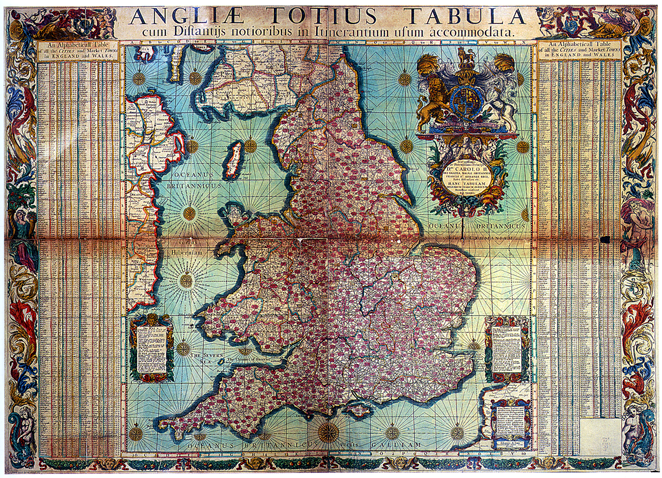
\includegraphics[width=0.65\textwidth]{images/adams1932john}
\caption{John Adams' Map of England. \cite{adams1932john} } \label{fig:historya}
}
\subfloat{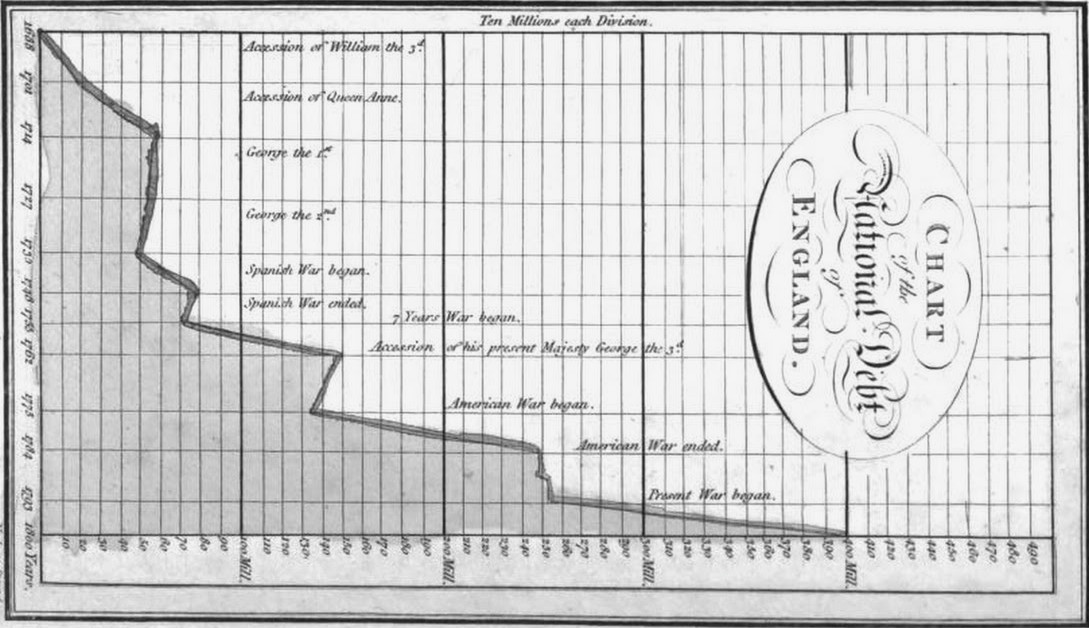
\includegraphics[width=0.47\textwidth]{images/playfairArea2}}~
\subfloat{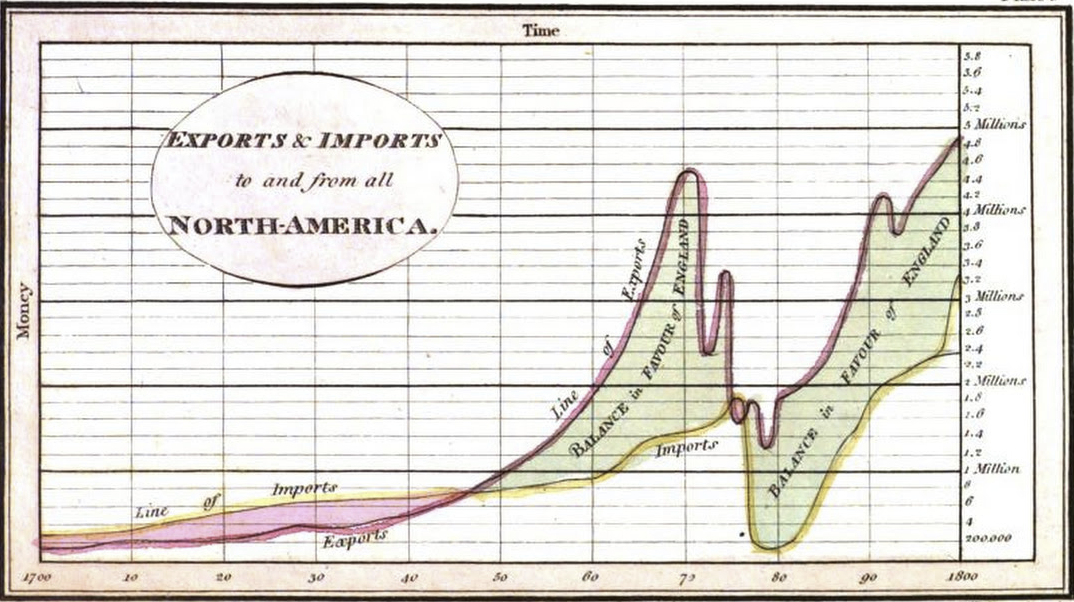
\includegraphics[width=0.485\textwidth]{images/playfairLine2}}\\
\subfloat{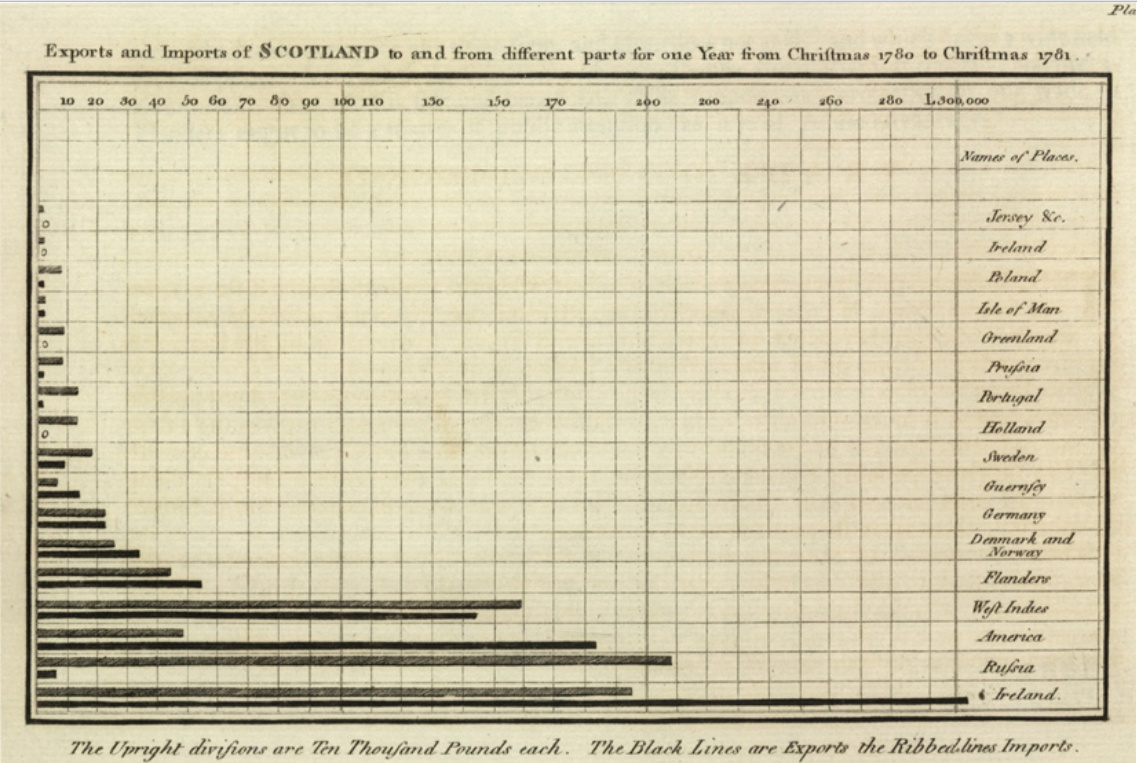
\includegraphics[width=0.42\textwidth]{images/playfairBar}}~
\subfloat{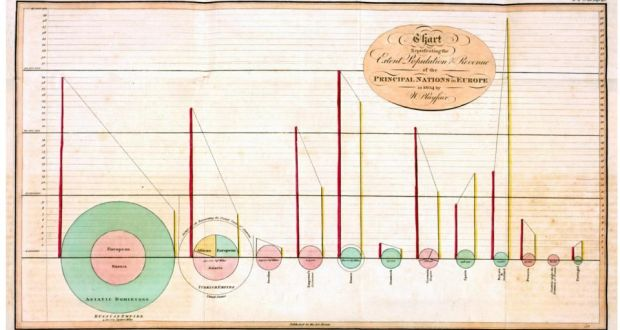
\includegraphics[width=0.53\textwidth]{images/playfairPie}}
\caption{Some of Playfair's original works. In order, Area chart and Line chart \cite{playfair1801commercial}, Bar chart \cite{playfair1786commercial}, and Pie chart \cite{playfair1801statistical}. }\label{fig:historyb}
\end{figure}

\section{Data Visualization}
Murray describes Data Visualization as "\emph{a process of mapping information to visuals}" \cite{murray2017interactive}, ideally something that improves over the raw data and proves a more comprehensible concept to a reader.
%Data Visualization is the exploration of mapping data to primitives in order to accurately present the data as a more flexible concept to a reader. 
Data can come from a potentially infinite number of sources. Designing robust techniques that handle data, as well as present meaningful interpretations that harbor large amounts of research and exploration into design are some goal of Data Visualization.

Evidence of Data Visualization is found as early as the 17th Century. In 1679, John Adams used Maps to depict the distance between different cities which could be used by travellers \cite{adams1932john} ( Figure \ref{fig:historya} ). These are comparable to modern network maps and gathered distance metrics with visual representation on a map.
Around the dawn of the 19th Century is considered the birth of modern data graphics\cite{friendly2001milestones}. William Playfair played an essential role in the history of visualization, known as the inventor of many common visual designs such as the bar chart, line chart, area chart, and pie chart \cite{playfair1786commercial,playfair1801commercial, playfair1801statistical}. See Figure \ref{fig:historyb}. 

Data visualization has only become more intrinsic to data analysis, with an increasing number of books being published on the topic \cite{rees2019survey}. In order to focus the discussion, we only discuss the related sub-fields that enable natural transition between Data Visualization and our thesis topic. Refer to \ref{fig:breakdown} for a visual breakdown.

\begin{figure}[t]
\centering 
\Centerstack{
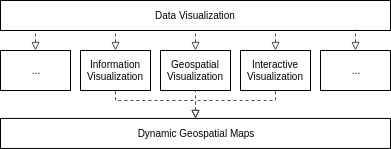
\includegraphics[width=0.58\textwidth]{images/ch1/SubjectDefinition2}}~
\Centerstack{
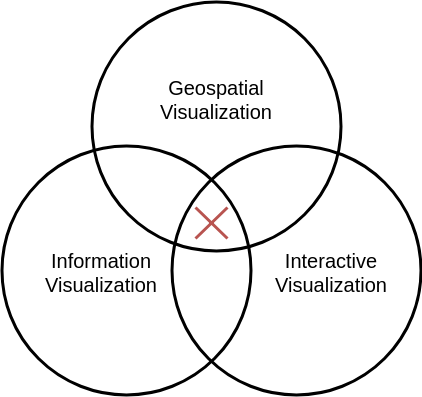
\includegraphics[width=0.28\textwidth]{images/ch1/venn1}}
\caption{A breakdown of the relevant fields discussed in the paper. In the form of (a) a relationship diagram and (b) a venn diagram.  Field selections is guided by Keim et al.\ \cite{ward2015interactive}} \label{fig:breakdown} 
\end{figure}

\subsection{Information Visualization}
Information visualization (InfoVis) is a sub-field of Data Visualization that focuses on abstract representation of data. InfoVis uses data and calculates or assigns a new abstract context to represent information to a user. Because of this, InfoVis provides a large range of unique techniques that can seem almost unrelated. We provide a few examples:\\
\textbf{Treemap: }A treemap is a representation of hierarchical data. By assigning the area of a treemap to the value an area holds, and applying this per hierarchy level, Johnson and Schneiderman created a space-filling algorithm \cite{johnson1991tree}. See Figure \ref{fig:treemap}. The treemap has become popular amongst visual analysts, with the main algorithm tweaked for many visual designs such as squarified \cite{bruls2000squarified}, strip \cite{bederson2002ordered}, and slice and dice \cite{shneiderman2001ordered}, and is used with many hierarchical datasets such as time \cite{roberts2016interactive}.

\begin{figure}[b]
\subfloat[Nested Treemap]{
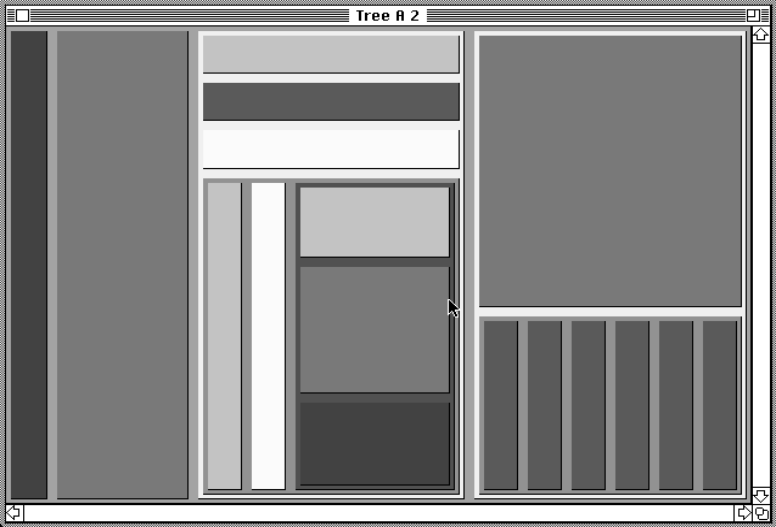
\includegraphics[width=0.4\textwidth]{images/ch1/nestedTreemap}}~
\subfloat[Non-Nested Treemap]{
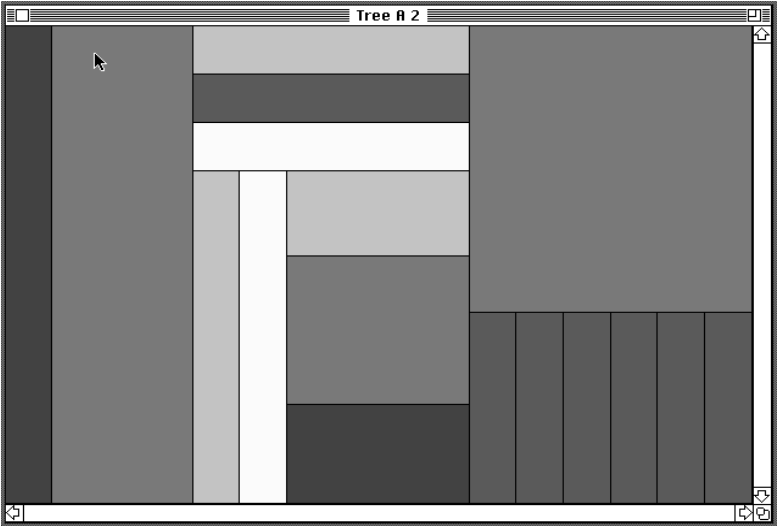
\includegraphics[width=0.4\textwidth]{images/ch1/treemap}}
\caption{The early treemap designs \cite{johnson1991tree}. } \label{fig:treemap}
\end{figure}

\begin{figure}[t]
\centering
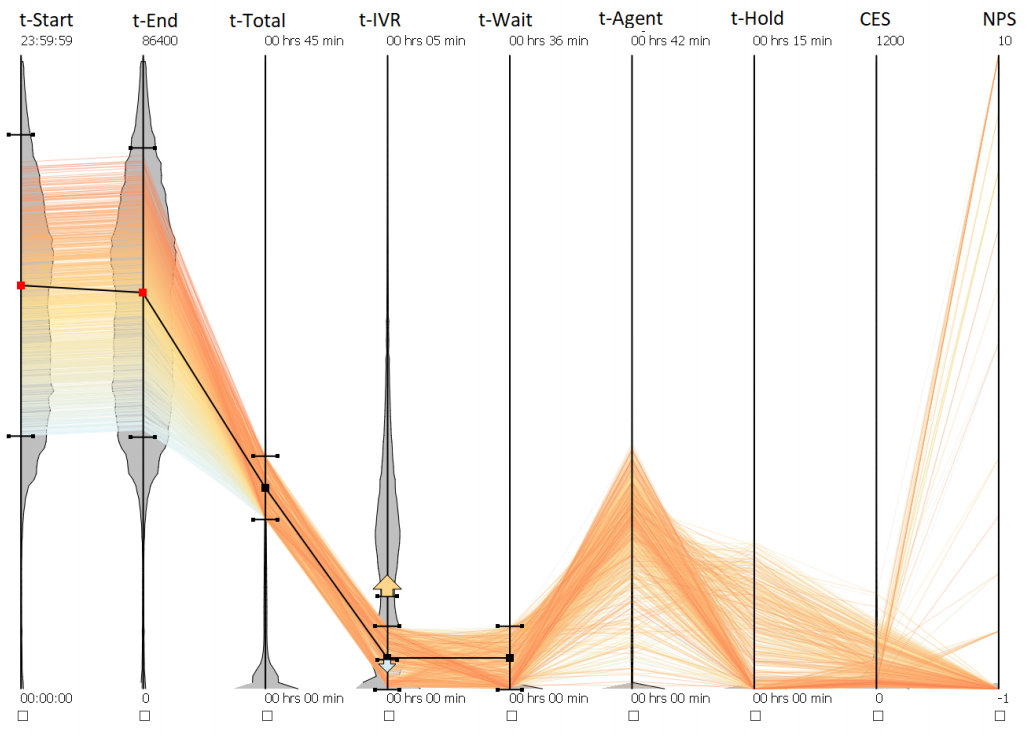
\includegraphics[width=0.5\textwidth]{images/ch1/pc2}
\caption{A typical example of a parallel coordinate, courtesy of Roberts et al. \cite{roberts2018smart}. } \label{fig:pc}
\end{figure}
\noindent
\textbf{Parallel Coordinates: } Parallel Coordinates are high dimensional representations of multivariate datasets used to search for relationships between attributes of data. For a standard parallel coordinate plot, each dimension is represented by a vertical axis, where the line represents the data range for the dimension. Each data record is assigned a polyline which connects each dimension in the range that represents eachattribute. The parallel coordinate was created by Inselberg \cite{inselberg1985plane}. See Figure \ref{fig:pc}.

\noindent
\textbf{Graphs: } Graphs are a large subset of InfoVis due to their utility. Graphs are used to represent connections or interfacing between objects. They can be used to visualize clusters or networks and flow in abstract space. Figure \ref{fig:graph} presents a collaboration diagram created to present how a class (created for later techniques) interacts with other classes. 

\begin{figure}[b]
\centering
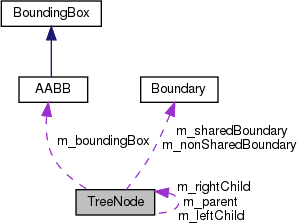
\includegraphics[width=0.5\textwidth]{images/ch1/graph}
\caption{A collaberation diagram created to present how a class interacts with other classes. This graph shows TreeNode holds three TreeNode objects, two Boundary objects, and an AABB, of type BoundingBox. Refer to \ref{chap:softdev}.} \label{fig:graph}
\end{figure}


\subsection{Geospatial visualization}
Geospatial visualization differs from InfoVis by incorporating spatial context as a geographical representation. The benefits of Geospatial visualization are with recognizability to the general public. However, their static nature can become an issue. We present some examples of geospatial visualization. 


\noindent
\textbf{Choropleth Map:} Choropleth maps are one of the oldest geographic visualization types \cite{dupin1827carte}. A choropleth map uses a standard geographical map split into administrative areas where each administrative area uses a visual mapping technique (such as color) to present associated values. The choropleth map is an integral part of Chapter \ref{chap:dcm} and is discussed more in detail there. See Figure \ref{fig:geo}(left).

\noindent
\textbf{Symbol Maps:} A symbol map differs from the choropleth map by using a symbol to visualiz the value of specific locations rather than mapping straight to the area itself \cite{cabello2010algorithmic}. However, both are often used in unison. Many symbols maps use size to represent the value of the underlying area. See Figure \ref{fig:geo}(right).
%Cartogram
\vspace{1.2cm}

\begin{figure}[hb]
\centering
\subfloat[Choropleth]{
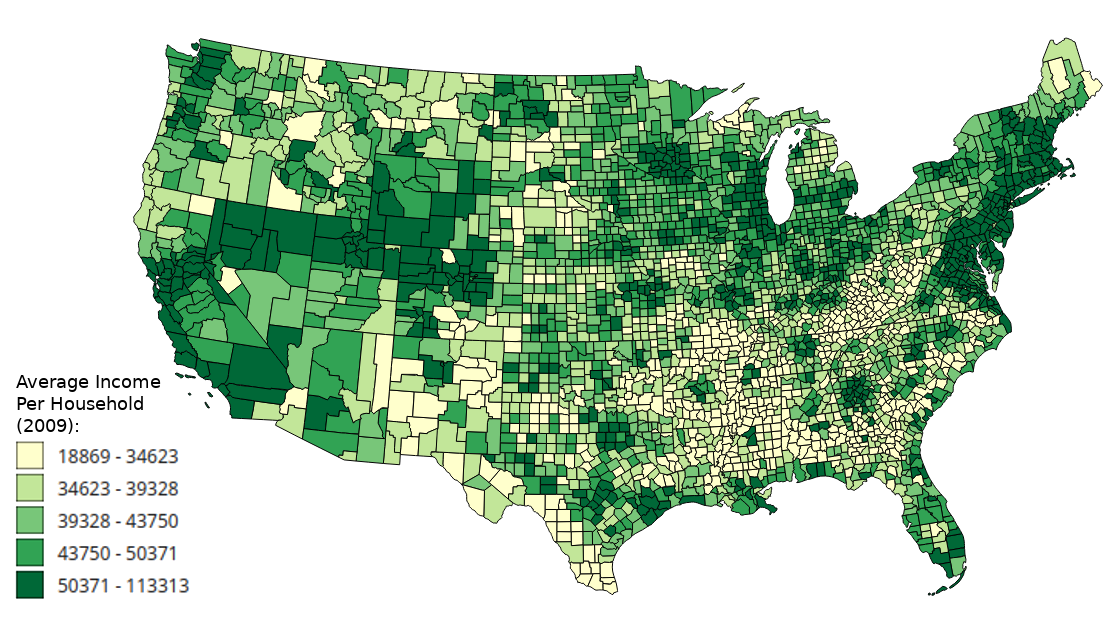
\includegraphics[width=0.63\textwidth]{images/ch1/choropleth}}
\subfloat[Minard's Symbol Map]{
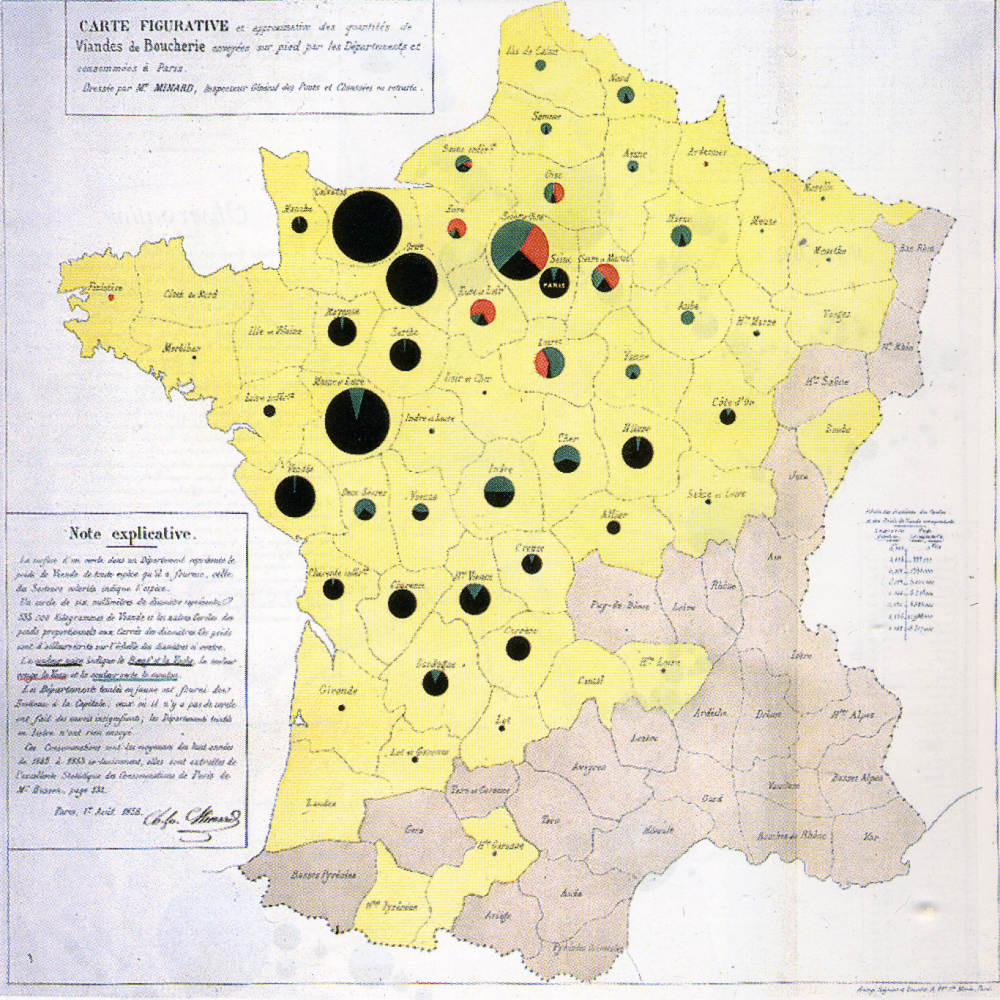
\includegraphics[width=0.33\textwidth]{images/ch1/minardsymbol}}
\caption{(left) A choropleth map depicting the average income of a household per US County. Generated using QGIS \cite{qgis2015qgis}. (right) Minard's famous example of a proportional symbol map, representing the cow consumption of France per area \cite{minard1858carte}. } \label{fig:geo} 
\end{figure}

\newpage

\subsection{Interactive Visualization}
Dynamic visualization differs from our previous two topics by acting as an enhancement for existing tools. We consider interactive visualization to represent critical areas of engagement with a user including animation, interaction techniques and adaptive views. All of these give the user control over how they want to manipulate or modify a visualization, whether that is through direct or indirect input. Interactive visualization is a leading theme throughout the thesis.

\subsection{Dynamic Geospatial Maps}
We review elements of information, geospatial, and dynamic visualization in order to create dynamic geospatial maps. We input raw geographic data, and present the data in Geospatial visualization form, however, we incorporate steps to manipulate the spatial context of the geographic data, using information visualization techniques. Finally, we enable dynamic visualization of our data through both direct and indirect manipulation of the view from our user. We provide a visual representation in Figure \ref{fig:topicbreakdown}.
\vspace{1.2cm}

\begin{figure}[hb]
\centering
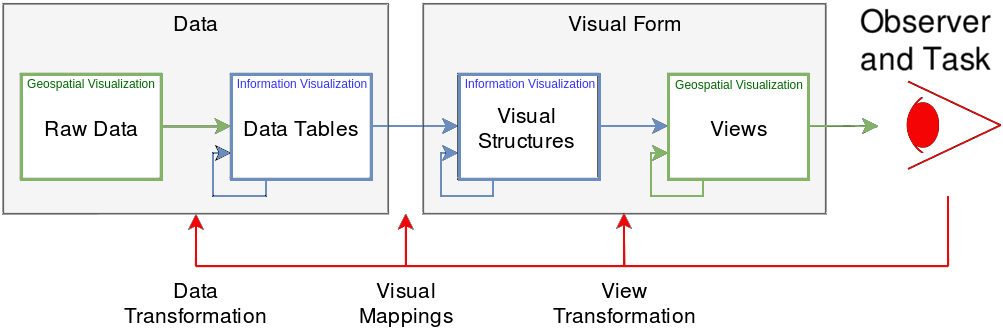
\includegraphics[width=1\textwidth]{images/ch1/TopicBreakdown2}
\caption{The information visualization pipeline introduced by Card et al \cite{card1999readings}. We highlight different sections to show how our three topics combine, green represents geospatial visualization, blue represents information visualization, and red represents dynamic visualization.                                                                                                                                                                                                                                                                                                                                                                                                                                                                                                                                                                                                                                                                                                                                                                                                                                                                                                                                                                                                                                                                                                                                                                                                                                                                                                                                                                                                                                                                                                               } \label{fig:topicbreakdown} 
\end{figure}

\newpage

\section{Challenges}
We consider three main challenges within our topic and our goals:
\begin{enumerate}
\item \textbf{Volume of Literature:} There is a large volume of literature in data visualization. In order to understand the needs of a user, we must clearly understand the existing in literature to figure out the current research topics that need to be examined. 
\item \textbf{Scalability:} Scalability is one of the major challenges we face in the field of visualization and is one we address in this thesis. Administrative areas of maps feature an assortment of complex boundaries, but the granularity of the areas can vary, leading to large amounts of complex borders. Administrative areas can be so small that it becomes difficult to interpret any data from them. For example, the United Kingdom holds over 180,000 areas of varying sizes, making an overview of the data recorded almost impossible without first transforming the data to a lower resolution. Our first and major challenge is to adress this challenge by using dynamic visualization to intuitively represent appropriately sized areas based on the user's view focus.
\item \textbf{Perception:} Our second challenge lies with the representation of areas. Cartograms already fill the niche of distorting area size to present administrative areas and their values. However, these techniques can either make it difficult or almost impossible to diagnose particular areas at just a glance. In order to avoid this, we need to produce a technique that minimizes any changes to the representation, offering an easier understanding of the underlying data.
\item \textbf{Multivariate Geospatial Data:} If we consider scalability as the breadth of data points, the we consider multivariate aspect as the depth per data point. If we want to present something a scalable we need to consider both of these aspect. In order to to do this, we need to create a multivariate geospatial map the presents meaningful data to the user.
\item \textbf{Performance:} Our final challenge lies with performance. The amount of computation necessary to update the display during rendering is counter-intuitive. We need to make sure that the technique we develop does not interfere with the user's exploration of the data.
\end{enumerate}

\section{Contribution}
The contributions of this thesis include:
\begin{enumerate}
\item \textbf{Volume of Literature:} The first Survey of Surveys covering the landscape of Information Visualization \cite{mcnabb2017sos}. The survey summarizes and classifies other survey papers in order to enable both newcomers and experienced researchers to obtain a greater understanding of the landscape of literature that has, and has not yet been published, as well as a broader understanding of future research challenges in the domain.
\item \textbf{Scalability: }The development of a novel technique for presenting choropleth maps at multiple levels of detail through user interaction \cite{mcnabb2018dynamic}. This is resolved by building a hierarchical data structure in which each area and its data is unified with one of its smallest neighbors recursively until only one polygon covers each contiguous region. The benefits are that the viewer can always view area-based data contained in the map regardless of how small any individual area becomes during interactive zooming.
\item \textbf{Perception:} An experiment to verify the relationship between choropleth maps, their underlying color map, and a user's perceivability \cite{mcnabb2018when}. We do this by testing a user's perception of color relative to an administrative area's size within a choropleth map, as well as user-preference of fixed-locale maps with enforced minimum areas based on the algorithm outlined in the Dynamic Choropleth Map algorithm.
\item \textbf{Multivariate Geospatial Data:} A multivariate map that uses scale-awareness to position multivariate glyphs and enables users to interact with both the map and glyphs to show meaningful data at different levels of detail \cite{mcnabb2019multivariate}. We discuss the algorithm pipeline for this process, as well as how the user can review and interact with the data. We present some user options to facilitate the exploration process and provide observations to support how the application can be used. We finish by reviewing the utility of the algorithm by looking at three case studies and comparing the map against an existing grid placement strategy. The result is a novel glyph placement solution to support multi-variate maps.
\end{enumerate}

\section{Thesis Structure}
The remainder of this thesis follows the following structure: In Chapter \ref{chap:SoS}, we present a survey of related work in the form of a survey of survey papers (SoS), that examines how research areas relate across different fields of Information Visualization. In Chapter \ref{chap:dcm}, we describe a novel technique to present choropleths at multiple levels of detail using a hierarchical data structure to unify administrative areas. Chapter \ref{chap:userStudy}, uses the algorithm presented in Chapter \ref{chap:dcm} to investigate how error relates to the scale of administrative areas on a map via a user study. The results provide guidance on the relationship between size and error, size and performance time, and some first steps in reviewing user preference in map design, concerning size. Chapter \ref{chap:MultivariateMaps} also builds on Chapter \ref{chap:dcm} by applying the choropleth algorithm to multivariate maps, using glyphs to present data for administrative areas. We improve upon the original method by adding clear transitions and uncertainty indicators, while also reviewing our algorithm against existing glyph-placement strategies. We look at some of the exciting aspects and challenges we ran into during the process of writing the thesis in Chapter \ref{chap:softdev}. Finally, in Chapter \ref{chap:conclusion} we draw our conclusion on the topic and discuss potential future work that can be applied to the topic of work. We also include an educational review discussing how to write a survey paper in Appendix \ref{chap:howTo}.